\documentclass[
	parskip=half,
	a4paper,
]{scrarticle}

\input{header.tex}
\addbibresource{../literature.bib}
\begin{document}

\title{Procedures for Hot Electron Measurements}
\author{Leon Oleschko}
\date{\dotdate\today}

\begin{titlepage}
    \sffamily
    \vspace*{3cm}
    {
        \fontsize{32}{32}
        \markieren{}{Hot Electron}{Thermal Emission}{Spectroscopy}
    }
    \vspace{.25cm}\\
    {
        \Large
        Leon Oleschko\\
        Supervised by Peter Baum
        \vspace{.05cm}\\
        \dotdate\today\\
        % \vspace{.25cm}\\
        % \normalsize
        Universität Konstanz
    }
    \vfill
    {
        \normalfont\normalsize

    }
    \vfill
    \begin{flushright}
        Available at \url{www.github.com/leoole100/projekt-praktikum}.
    \end{flushright}
\end{titlepage}

% {
% 	\sffamily
% 	\hypersetup{hidelinks}
% 	\tableofcontents
% }

\clearpage


\section{Introduction}

\clearpage
\section{Experimental Setup}
\begin{figure}[hb]
    \centering
    \includegraphics{figures/setup.pdf}
    \caption{Schematic of the experimental setup.}
    \label{fig:setup}
\end{figure}
The experimental setup, as designed by Leon Roob \cite{roob_thermal_2025}, is show schematically in \autoref{fig:setup}.
It is a broadband photoemission setup.

Firstly the laser is a Pharos \textbf{TODO} by Light Conversion with a wavelength of \SI{1030}{nm}, a FWHM Pulse width of \SI{250}{fs} and a repetition rate of \SI{100}{kHz}.
The beam is 4 axis stabilized and has a diameter of \textbf{TODO} \si{mm}, when it enters the experiment.
The lens \textsf{L} with a focal length of \SI{150}{mm} focuses the light on the sample with a diffraction limited spot size of $4 \lambda f / \pi D = $ \textbf{TODO}.

The sample is absorbing the laser pulse and emitting thermal radiation into the half sphere.
To collect and focus the broad band emission off-axis parabolic mirrors with  UV-enhanced aluminum coating are used (\textsf{PM}).
\textsf{PM1} with a focal length of \SI{50}{mm} is used to collect the emission and \textsf{PM2} with a focal length of \SI{101}{mm} is used to focus the light through a filter onto a bare multi-mode fiber end.

The used fiber is a QP200-2-SR-BX from Ocean Optics. A \SI{200}{\micro m} multi-mode fiber for transmission from $300-1100$\;\si{nm}.

To analyse the light a Acton SpectraPro 300i monochromator with a $150$\;lines/mm grating with a blazing wavelength of \SI{500}{nm} is used.
The light is detected using a Andor iXon$^\text{EM}$+ 897 EMCCD camera used in Vertical Binning mode as a line detector.

The lens \textsf{L}, the sample and the fiber end are mounted on 3 axis translation stages, to aid in focusing. The parabolic mirrors are fixed.

\section{Characterization of Noise Sources}
To be able to detect a the faint thermal radiation from the hot electrons it is necessary to optimize the signal-to-noise ratio (SNR) of the experiment.

The noise sources of the setup are mainly from the detector.
Variation in the laser output power are assumed to be comparatively small and ignored in the following discussion.

The detector used is a EMCCD camera as is common for spectroscopy. The manufacturer Andor has some documents that discuss the Optimisation of SNR \cite{andor_establishing_nodate,dr_jo_walters_sensitivity_2023}.

The simplest noise source is \textit{Readout Noise}. Every bin that is read out get's a constant noise from the CCD shifting and the analog to digital converter. For the high performance CCD camera used here this is in the order of \SI{1}{e^-} \cite{andor_ixonem_nodate}. It is measured to be in that range in \autoref{fig:dark_noise}.
This is applied per read out bin, not per pixel, leading to the use of hardware vertical binning.

\begin{figure}[hb]
    \centering
    \includegraphics{../analysis/figures/dark_noise.pdf}
    \caption{Dark noise as a function of sensor temperature and exposure time. The curve is fitted with an effective activation energy of $E = \SI{0.597(4)}{eV}$ and a constant readout noise of $\sigma_{\text{read}} = \SI{0.81(12)}{e^-}$.}
    \label{fig:dark_noise}
\end{figure}
Another noise source is \textit{dark current noise}. 
It is a results from thermal energy stochastically exciting electrons in the semiconductor of the detector. The noise this generates scales with temperature and time $N_\text{dark} \propto \exp(-E / k T) \cdot t_\text{exp}$. This is shown in \autoref{fig:dark_noise}.
For this reason scientific cameras are mostly cooled, here to \SI{-80}{\degreeCelsius}, such that this is insignificant for this setup.


Then there is is \textit{Clock Induced Charge Noise}, that scales with the electron multiplying gain in the detector and proportional to the signal. For this reason it is beneficial to deactivate the sensor gain, when the signal is significantly stronger that the readout noise \cite{andor_establishing_nodate}, like in this case.

The main resulting noise source is shot noise, such that the system is called shot noise limited.
\textbf{TODO}: It is still to be researched if the shot noise is per photon, or per electron.

\section{Efficiency and Flatness}
Not all light that is emitted from the sample is detected.
The amount of light that is detected can be considered the efficiency of the setup. This is not a constant across wavelength.

The mirrors and the fiber are selected to be reasonably flat across the detected spectrum, so they just change the efficiency of the setup by a constant amount.

\begin{figure}[hb]
    \centering
    \includegraphics{../analysis/figures/filter.pdf}
    \caption{Efficiency of various components and filters used in the setup.}
    \label{fig:efficiency}
\end{figure}
The filter to block the excitation laser can be measured. This is shown for two different filters in \autoref{fig:efficiency}. The KG3 Filter is a filter made by SCHOTT to absorb Infrared it has a shallow transmission edge, cropping the expected thermal emission.
The HR filter is presumably a Edmund optics highly reflective dielectric short pass filter. Details are not know, as it was just labeled HR.

More interesting are the efficiency curves of the detector and the grating, as they are not easily measured. In figure \autoref{fig:efficiency} the quantum efficiency from the manufacturer is plotted for the camera. The efficiency of the the grating is more complicated, as it depends on the exact parameters of the blazed grating. Here a simple model from \cite{barker_ripple_1984} is used.



\subsection{Calibration}
To determine the efficiency curve of the spectrometer it has to be calibrated.

The easiest way is to use a white light source with a known spectrum, and transfer the calibration from the calibration lab, that was used for calibrating the light source.

\begin{figure}[hb]
    \centering
    \includegraphics{../analysis/figures/efficiency_different.pdf}
    \caption{Same spectrum recorded with different instruments.}
    \label{fig:calibration}
\end{figure}
A different approach would be to get a calibrated spectrometer and use that one to calibrate a light source. This was tried with a deuterium halogen lamp (DH-2000-BAL from ocean optics), with multiple different ocean optics USB spectrometers.
The recorded spectra are shown in \autoref{fig:calibration}. 
As the spectrometer have different sensitivities, the Intensity axis had to be scaled differently for each spectrometer. But the instrument don't agree, which shows that calibrating to more trusted instrument is necessary.


\clearpage
\section{Data Analysis and Spectral Modeling}

\clearpage
\section{Conclusion}

\clearpage
\printbibliography

\end{document}